% C2GES original-title reconstruction, P60 revision after a 20-paper Applied Sciences benchmark.
% Scientific evidence remains the independently audited v0.3.1 post-audit corrective run only.
\documentclass[applsci,article,submit,moreauthors]{Definitions/mdpi}
\firstpage{1}
\makeatletter\setcounter{page}{\@firstpage}\makeatother
\pubvolume{1}\issuenum{1}\articlenumber{0}\pubyear{2026}\copyrightyear{2026}
\datereceived{}\daterevised{}\dateaccepted{}\datepublished{}
\newcommand{\cges}{C\textsuperscript{2}GES}
\setlength{\headheight}{20pt}
\AtBeginDocument{\pdfstringdefDisableCommands{\def\cges{C2GES}}}

\Title{C\texorpdfstring{\textsuperscript{2}}{2}GES: Structure-Aware Extractive Summarization of Long Power-System Technical Reports with Typed-Path Graphs}
% ORCID: none declared for either author on 24 August 2026; per the MDPI template, ORCID commands are omitted.
\Author{Bijing Liu $^{1,2}$ and Yong Yang $^{1,2,}$*}
\AuthorNames{Bijing Liu and Yong Yang}
\address{$^{1}$ \quad NARI Group Corporation (State Grid Electric Power Research Institute), Nanjing 211106, Jiangsu Province, China;\\
$^{2}$ \quad Beijing Kedong Electric Power Control System Co., Ltd., Beijing 100080, China}
\corres{Correspondence: yangyong1@sgepri.sgcc.com.cn}

\abstract{Evidence about a power-system event is often dispersed across long technical reports, so relevance-only extracts may not form a coherent engineering account. We present \cges{}, a deterministic framework that combines centroid lexical relevance, transparent text roles, a typed sentence graph, node-deletion path participation, and source-page traceability. We evaluated seven conditions at two budgets on 12 development and 15 test reports from the North American Electric Reliability Corporation. The unrenormalized coefficient-removal comparison achieved the highest mean ROUGE-L. Full \cges{} reached ROUGE-L F1 values of 0.1060 and 0.1276 and exceeded Semantic-MMR and TextRank at equal unit budgets, but its extracts were 54--63\% longer. Under development-derived word caps, every Full-minus-baseline series-cluster interval crossed zero, and no exact comparison survived Holm adjustment. The path term changed most selected sequences without improving the predefined endpoint, while development-only calibration selected zero path weight in all 12 folds. The study therefore establishes an auditable, source-linked implementation and a negative result for the current path component. It does not establish a length-controlled advantage or operational reading benefit. Evaluation on unseen reports by qualified experts remains necessary.}
\keyword{extractive summarization; typed textual proxy graph; structural perturbation; power-grid reports; NERC; auditable evaluation}
\featuredapplication{\cges{} is designed to support source-linked navigation of long power-system technical reports by selecting passages associated with condition, event, impact, and mitigation roles. It is intended for analyst support: extracted passages remain linked to their original pages, and operational use requires validation on maintenance records and expert review.}

\begin{document}

\section{Introduction}

Power-system reliability and event-analysis reports often extend across hundreds of pages. Evidence about an initiating condition, a trigger, system propagation, consequences, and corrective action may appear in different sections and coexist with tables, standards language, recommendations, and appendices. Engineers reviewing such material need more than a list of individually prominent sentences. They need a compact route through structurally complementary passages and a reliable way to return to the source.

Extractive summarization is attractive in this setting because it preserves the wording and location of selected passages. Position, centroid-style lexical relevance, graph centrality, and semantic diversity provide useful ranking signals \cite{zhong2020extractive,bi2021aredsum,liu2021unsupervised,mihalcea2004textrank,reimers2019sentencebert}. These signals, however, do not necessarily distinguish the roles that passages play in an engineering account. A highly central passage may repeat background information, whereas a less central passage may contain the only mitigation or consequence needed to interpret an event.

Graph-based summarizers model relationships among sentences through learned graphs, hypergraphs, or structural filtering \cite{siragusa2022sentencegraph,onan2024mches,hark2025mis}. Power-domain language studies use entity--relation extraction and knowledge graphs to organize fault, alarm, and inspection evidence \cite{liu2022powerfault,ma2025alarm,zgg2026bridge}. \cges{} links these lines of work in an engineering-oriented formulation: candidate units receive transparent textual roles, compatible roles form typed paths, and path participation is combined with relevance, graph salience, position, and redundancy control. Each selected unit remains linked to its original report page.

The study uses complete public reliability, disturbance, event-analysis, recommendation, and assessment reports from the North American Electric Reliability Corporation (NERC). NERC guidance on the attributes of quality event-analysis reports provides the institutional context for this report family \cite{nerc2015qualityreport}. These reports contain event narratives and corrective lessons but are not utility work orders, inspection records, or field-maintenance narratives. The corpus is therefore treated as a maintenance-oriented technical-report proxy. Twelve reports support development, and 15 reports form the retained test set. All candidates are drawn from report pages outside the official Executive Summary, which is used only as the reference for automatic evaluation.

Three questions organize the evaluation. \textit{RQ1} asks how the seven evaluated conditions compare on the selected NERC corpus at fixed extraction-unit budgets and how differences in output length limit system-level interpretation. \textit{RQ2} asks whether the typed path-deletion term improves ROUGE-L or redundancy relative to the otherwise fixed unrenormalized coefficient-removal comparison. \textit{Exploratory RQ3} asks how consistently the term changes candidate scores and selected sequences across reports and budgets, and whether development-only coefficient calibration supports a nonzero path-deletion weight.

The paper makes three contributions. First, it introduces a deterministic, role-conditioned typed-path framework that selects structurally complementary passages and preserves their source pages. Second, it evaluates seven conditions at two extraction-unit budgets on complete NERC reports, with report-level pairing and explicit output-length diagnostics. Third, it separates system behavior from component benefit. Full \cges{} had higher observed ROUGE-L than the external baselines at equal unit budgets, but it also produced longer outputs. The unrenormalized coefficient-removal comparison was slightly better, and development calibration did not support a positive path weight. The current path integration is therefore a diagnosed design limitation rather than a validated performance mechanism. These findings concern the selected technical-report proxy and do not establish performance on operational maintenance records.

\section{Related Work}

\subsection{Extractive Technical-Document Summarization}

Extractive methods rank source sentences using position, document-centroid similarity, graph centrality, learned salience, or redundancy-aware relevance \cite{zhong2020extractive,bi2021aredsum,liu2021unsupervised}. Lead and centroid methods remain useful controls, while TextRank provides a widely used graph-ranking reference \cite{mihalcea2004textrank}. Dense sentence representations extend lexical matching and support semantic relevance--diversity selection \cite{reimers2019sentencebert}. Holding candidates, references, preprocessing, and extraction-unit budgets constant allows these ranking principles to be compared within one report corpus, although representation and tuning opportunities still differ.

Long technical documents add layout and discourse problems that are less prominent in short news articles. Bug-report summarization, for example, must distinguish problem statements, observed behavior, diagnostic discussion, and resolution-oriented passages \cite{koh2022bugreport}. Multi-document methods must likewise balance common content against source-specific evidence \cite{zhang2024tomds}. NERC reports combine long narrative sections with tables, standards language, recommendations, and appendices. This motivates a selector that considers both sentence relevance and the role of a passage in the report's engineering account.

\subsection{Graphs, Semantic Ranking, and Causal Language}

Graph summarizers model relations among sentences, entities, topics, or discourse units \cite{wang2020heterogeneous,cui2020enhancing,jing2021multiplex}. Learned sentence graphs, contextual hypergraphs, independent-set filtering, and heterogeneous long-document graphs all extend isolated relevance scoring \cite{siragusa2022sentencegraph,onan2024mches,hark2025mis,bugueno2025graphlss}. \cges{} takes a complementary approach. It uses fixed lexical roles and deterministic typed-path enumeration so that the contribution of each score channel and selected sentence can be inspected.

The graph is rebuilt for each report and does not store a persistent asset ontology. Its node-deletion term measures how much qualified textual-path utility is lost when one sentence node is removed. This is a structural sensitivity feature, not an alternative physical event. Causal NLP distinguishes language association from intervention and counterfactual identification \cite{feder2022causal,du2022ecare}; accordingly, the present method is described as causal-chain-inspired only in the sense of its condition--event--impact--mitigation role progression. The remainder of the paper uses the more precise term \emph{path-deletion term}.

\subsection{Power-Grid Text Analytics}

Grid language technologies cover infrastructure analysis, digital twins, supervised entity--relation extraction, and persistent knowledge graphs \cite{xie2022massively,hamann2024foundation,madabhushi2023survey,srinivasan2023artificial,ranawaka2024leveraging,meng2023gridfield}. Power-fault, line-loss, and alarm-tracing graphs organize entities or events \cite{liu2022powerfault,li2024lineloss,ma2025alarm}. Maintenance-oriented retrieval and knowledge-graph studies use equipment or inspection records and sometimes include annotation or practitioner evaluation \cite{cao2024coalmaintenance,zgg2026bridge,dimaggio2025predictivemaintenance}. Relation-extraction methods similarly predict supervised entity--relation labels \cite{li2025moere,she2025clear}.

\cges{} addresses a different level of analysis: it ranks passages from a complete report while preserving source locations and encouraging complementary textual roles. Table~\ref{tab:related-comparison} positions this formulation against adjacent Applied Sciences studies. The contribution evaluated here is the integration of deterministic role evidence, typed-path participation, source-linked extraction, and a strict component ablation. The study claims neither absolute priority over adjacent methods nor a performance benefit from the current path-deletion term.

\begin{table}[H]
\caption{Positioning against selected Applied Sciences studies with related structural or power-domain objectives.}
\label{tab:related-comparison}\centering\scriptsize
\begin{tabularx}{\textwidth}{p{2.5cm}p{2.4cm}p{2.5cm}p{2.5cm}X}
\toprule
Study family & Primary object & Structural mechanism & Evaluation emphasis & Difference from this study\\
\midrule
Sentence Graph Attention / MCHES \cite{siragusa2022sentencegraph,onan2024mches} & General-domain documents & Learned sentence graph or contextual hypergraph & Summary metrics on benchmark corpora & Learned semantic representations; no NERC proxy or node-deletion ablation\\
Graph MIS + LLM \cite{hark2025mis} & DUC and CNN/DailyMail documents & Independent-set filtering and graph metrics & ROUGE and computational efficiency & Different graph objective, corpora, and generation components\\
Bug-report summarization \cite{koh2022bugreport} & Software issue reports & Learned sentence significance & Technical-artifact summary quality & Similar long technical discourse, but different roles, references, and domain\\
Power fault/alarm graphs \cite{liu2022powerfault,ma2025alarm} & Power-domain entities and events & Ontology/KG extraction and graph tracing & Entity, relation, or tracing performance & Structured knowledge construction rather than report-level extractive summarization\\
Maintenance KG and retrieval \cite{cao2024coalmaintenance,zgg2026bridge} & Equipment or inspection records & LLM retrieval or ontology-constrained extraction & Retrieval, annotation, manual audit, or practitioner utility & Title-concordant data and human assessment; no comparable extractive ablation\\
\cges{} & Selected NERC technical reports & Deterministic role graph and typed-path deletion & Executive-Summary overlap, paired contrasts, and length diagnostics & Report-level extractive selection with source-linked outputs and a strict component ablation\\
\bottomrule
\end{tabularx}
\end{table}

\section{Materials and Methods}

\subsection{Task Formulation and System Overview}

Let report $D=\{s_1,\ldots,s_n\}$ contain non-summary candidate extraction units. For budget $K\in\{5,10\}$, method $m$ returns $\hat{Y}_{m,K}\subseteq D$, with $|\hat{Y}_{m,K}|=\min(K,n)$. The selected units are restored to source order. The official Executive Summary is used only as the reference and is never candidate input.

ROUGE-1, ROUGE-2, and ROUGE-L F1 quantify lexical overlap between the extract and that Executive Summary \cite{lin2004rouge}. The acronym ROUGE denotes Recall-Oriented Understudy for Gisting Evaluation. ROUGE-L is the predefined primary endpoint; redundancy is a descriptive secondary outcome. These measures characterize reference overlap and lexical repetition rather than expert-assessed completeness or operational usefulness.

Figure~\ref{fig:algorithm} summarizes the deterministic pipeline. Complete reports first pass candidate and reference-separation gates. Each retained candidate receives five lexical role scores and contributes, when a unique role is assigned, to a typed sentence graph. Relevance, role, graph, path-deletion, and position channels form a base score. The selector reserves available evidence from three role groups before filling the remaining budget with a redundancy-aware greedy rule. Selected passages are restored to source order and retain identifiers that resolve to the original pages.

\begin{figure}[H]
\centering
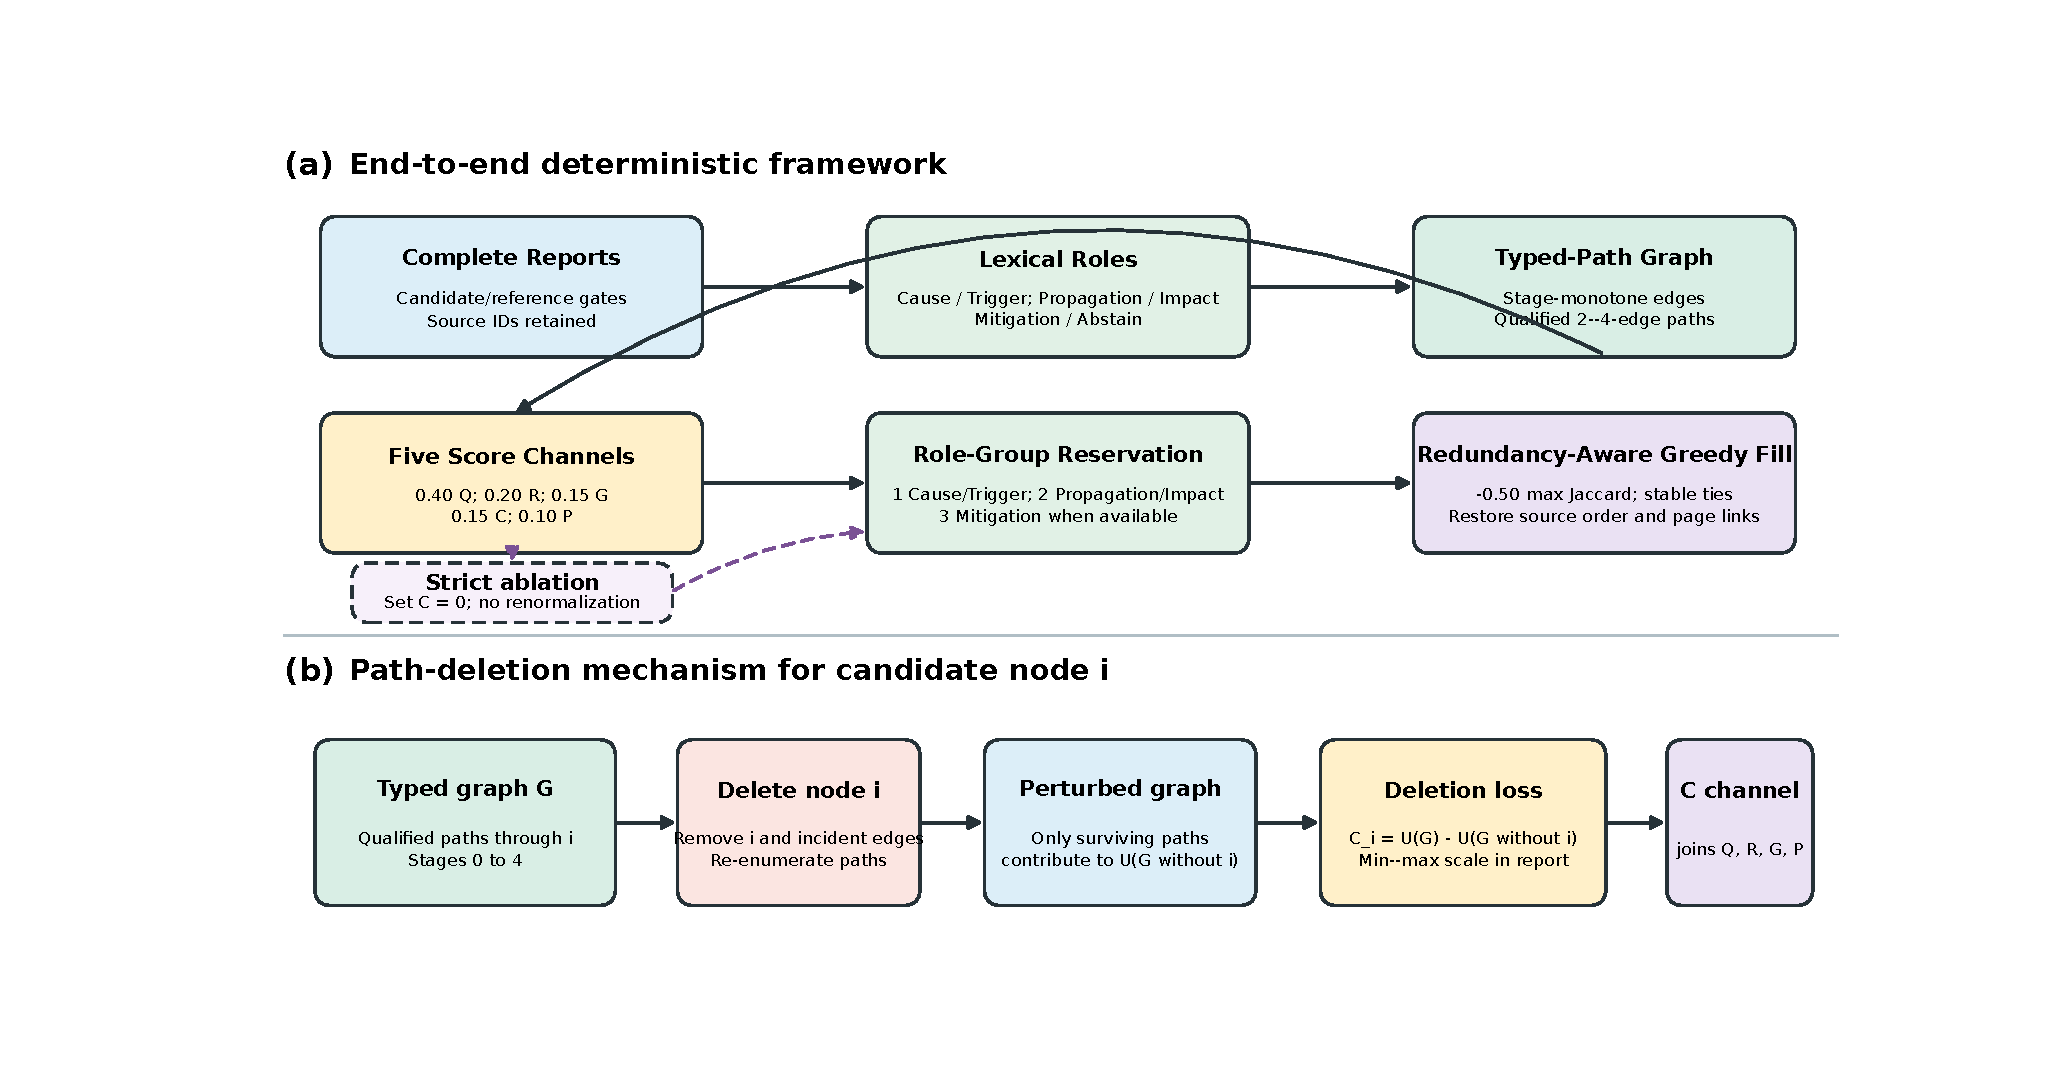
\includegraphics[width=\textwidth]{figures/fig01_algorithm_dual_panel.pdf}
\caption{Deterministic \cges{} pipeline and path-deletion mechanism. \textbf{(a)} Complete reports pass candidate and reference-separation gates; retained passages receive lexical roles and form a typed textual graph. The five score channels feed an ordered role-group reservation followed by redundancy-aware greedy filling. The unrenormalized coefficient-removal comparison sets $C$ to zero without renormalizing the remaining coefficients. \textbf{(b)} For candidate node $i$, path-deletion loss removes $i$, recomputes qualified-path utility, and takes $C_i=U(G)-U(G\setminus i)$.}
\label{fig:algorithm}
\end{figure}

The unit of analysis is the report. Candidate units within a report share topic, vocabulary, layout, and reference-summary content and are not treated as independent observations. Candidate-level quantities drive selection, whereas paired differences and composition intervals use the 15 report-level observations.

\subsection{Corpus Construction and Reference Separation}

The corpus builder inspected 40 complete public PDFs covering 3200 declared pages. It retained 27 reports and excluded 13 before outcome computation; 12 retained reports were assigned to development and 15 to test. Figure~\ref{fig:data-flow} summarizes this construction, and Supplementary Table~S1 provides the non-verbatim sampling frame and exclusion reasons.

Inclusion required a complete readable PDF, a detectable summary reference, a non-empty post-summary candidate region, and passage of the predefined extraction-quality gates. Exclusion was decided before outcome computation and remained visible in the inventory. This procedure reduces discretionary removal after observing ROUGE values, but it also changes the estimand: the results concern reports that satisfy the builder's document and reference requirements, not every NERC publication. An operationally important report without a conventional Executive Summary remains outside the present automatic evaluation.

Development and test assignment was performed at report level so that sentences from one source could not cross partitions. Reference-summary text was used only for development scoring or final evaluation, never as a candidate. The builder preserved report ID, page interval, source order, and candidate ID so that every downstream score could be joined directly to its extraction record.

\begin{figure}[H]
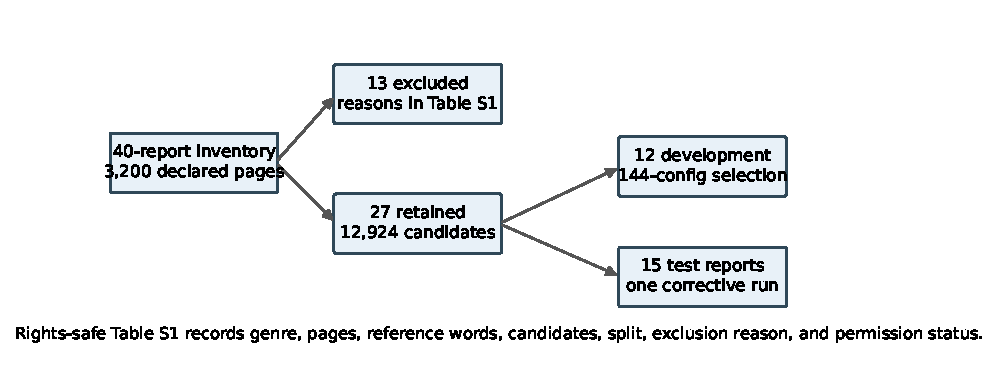
\includegraphics[width=\textwidth]{figures/fig02_dataset_flow.pdf}
\caption{Corpus construction and partitioning. Boundary and extraction-quality gates retained 27 of 40 complete PDFs. Twelve reports supported configuration selection, and 15 formed the retained test set.}
\label{fig:data-flow}
\end{figure}

Candidates begin after a conservatively detected Executive Summary boundary, and no fixed sentence cap is applied. The builder produced 12,924 candidates, with 51--1898 per report. Rebuilding the corpus found no reference/body page overlap, normalized exact candidate/reference match, or normalized common substring of at least 50 characters. These checks prevent direct reference leakage caused by page or extraction errors; legitimate paraphrase and facts repeated in the report body remain part of the task.

\subsection{Sentence Roles and Typed Textual Proxy Graph}

Each candidate receives lexical evidence for root cause, trigger event, propagation or response, impact, and mitigation. Positive top-score ties lead to abstention rather than resolution by a fixed role order; all 111 development ties received no dominant role and no incident directed edge. The v0.3 selector received no reference role labels.

For each role, the implementation counts predefined cue classes and divides all non-negative scores for that role by the largest score in the report. The role channel $R_i$ is the maximum of these five unit-scaled values. A dominant role is assigned only when one positive role score is uniquely maximal. An all-zero vector or equal positive maximum yields abstention. An abstaining unit remains eligible for selection through the non-role channels but contributes no typed-path edge.

Table~\ref{tab:taxonomy} gives the executable taxonomy and representative substring-based lexical cues. The system does not detect grammatical scope, factual status, or document-level coreference.

\begin{table}[H]
\caption{Executable role and transition taxonomy. These are lexical text proxies, not expert labels or physical relations.}
\label{tab:taxonomy}\centering\small
\begin{tabularx}{\textwidth}{p{2.2cm}XX}
\toprule
Role & Representative cue classes & Permitted outgoing transitions\\
\midrule
Root cause & cause, due-to, failure, and protection-setting terms & trigger; propagation or response; mitigation\\
Trigger event & fault, outage, initiation, trip, and fire terms & propagation or response; impact\\
Propagation or response & trip, voltage, frequency, islanding, load-shed, reserve, and flow terms & impact\\
Impact & quantities with grid units, customer, load, loss, and unavailability terms & mitigation\\
Mitigation & recommendation, corrective, preventive, and standard terms & none\\
Abstention & no positive cue, or more than one equal positive maximum & none\\
\bottomrule
\end{tabularx}
\end{table}

A directed edge is allowed only for predefined stage-monotone role transitions whose candidate positions differ by at most 12. The implementation maps root cause, trigger event, propagation or response, impact, and mitigation to stages 0, 1, 2, 3, and 4, respectively. Let $d_{ij}=|\operatorname{pos}(i)-\operatorname{pos}(j)|$, let $J_{ij}$ be token-set Jaccard overlap, and let $r_i,r_j\in[0,1]$ be the unit-scaled dominant-role scores. The edge weight is
\[
w_{ij}=\operatorname{round}_{12}\!\left[0.45\exp(-d_{ij}/5)+0.30J_{ij}+0.25\min(r_i,r_j)\right].
\]
Thus $w_{ij}\in[0,1]$. Min--max scaled weighted degree within the report forms graph salience $G_i$.

The edge gate has semantic and positional components. The source and target roles must appear in the stage-monotone transition set in Table~\ref{tab:taxonomy}, and their candidate indices must lie within the 12-position horizon. The implementation uses absolute positional distance and therefore does \emph{not} require the source-role unit to occur earlier in document order; edge direction follows the role transition rather than chronology. The weight rewards proximity, lexical continuity, and confident role assignments. A high weight therefore means ``nearby, lexically connected, and compatible with the predefined role progression''; it does not indicate that a domain expert verified the relation or its temporal order.

These choices make the graph sparse and document specific. Sparse construction limits path enumeration and improves inspectability, while document-specific normalization avoids comparing raw node degrees across reports of very different size. The design also creates known blind spots. A causal statement whose evidence and consequence are separated by more than 12 candidates cannot form an edge; a relation expressed through coreference may have low token overlap; a role-compatible edge may point against document chronology; and a valid sentence with two equally strong role cues abstains. These are algorithmic consequences rather than post hoc explanations of individual outcomes.

\subsection{Typed Path-Deletion Structural Perturbation}

Let $\mathcal{P}(G)$ be the set of simple, stage-monotone paths with two to four edges beginning at a root-cause or trigger node and ending at an impact or mitigation node. For path $p$,
\begin{equation}
\operatorname{strength}(p)=\left(\prod_{e\in p}w_e\right)^{1/|p|}\frac{\max\operatorname{stage}(p)-\min\operatorname{stage}(p)}{4}.
\end{equation}
The graph utility and raw deletion score are
\begin{equation}
U(G)=\sum_{p\in\mathcal{P}(G)}\operatorname{strength}(p),\qquad
C_i=U(G)-U(G_{-i})=\sum_{p\ni i}\operatorname{strength}(p).
\end{equation}
Unlike weighted degree, $C_i$ depends on qualified multi-edge path membership, role order, and the geometric mean of edge weights. A synthetic unit-test counterexample gives two nodes equal weighted degree but unequal qualified-path membership. Unit tests verify deletion-loss equality, deterministic scaling, cache equivalence, and fail-closed work limits. These checks establish software and mathematical non-identity, not physical causality or effectiveness.

The functional has three design properties under a fixed qualified-path set: non-negativity when edge weights are non-negative; nullity for a node that belongs to no qualified path; and additivity over the qualified paths that contain the deleted node. More precisely, if deleting node $i$ removes exactly those paths containing $i$ and does not change the weights of paths that remain, then $C_i=\sum_{p\ni i}\operatorname{strength}(p)$. This proposition is an accounting identity for a fixed textual graph, not a causal-identification theorem. It can fail as a model of semantic influence when deletion would change role assignments, coreference, discourse interpretation, or the weights of surviving relations; the implemented perturbation intentionally holds those quantities fixed.

Table~\ref{tab:toy-path} provides a synthetic walk-through that is independent of the experimental corpus. Consider five source-ordered nodes with roles root cause, trigger, propagation, impact, and mitigation and four compatible edge weights. The four qualified paths that begin at the root-cause or trigger node and end at impact or mitigation have strengths 0.566964, 0.741559, 0.367423, and 0.542282 under Equation~(1), giving $U(G)=2.218228\approx2.218$. Deleting the propagation node removes all four paths, so $C_{q}\approx2.218$; deleting the root-cause node removes only the two paths that start there, so $C_{r}=1.308523\approx1.309$. The example shows why path participation and stage span matter beyond local edge totals.

\begin{table}[H]
\caption{Synthetic typed-path example used only to explain the implemented computation; it is not an experimental observation.}
\label{tab:toy-path}\centering\small
\begin{tabular}{llll}
\toprule
Nodes on path & Edge weights & Stage-span factor & Path strength\\
\midrule
$r\rightarrow t\rightarrow q\rightarrow i$ & 0.8, 0.6, 0.9 & $3/4$ & 0.567\\
$r\rightarrow t\rightarrow q\rightarrow i\rightarrow m$ & 0.8, 0.6, 0.9, 0.7 & $4/4$ & 0.741\\
$t\rightarrow q\rightarrow i$ & 0.6, 0.9 & $2/4$ & 0.367\\
$t\rightarrow q\rightarrow i\rightarrow m$ & 0.6, 0.9, 0.7 & $3/4$ & 0.542\\
\bottomrule
\end{tabular}
\end{table}

The equality $C_i=\sum_{p\ni i}\operatorname{strength}(p)$ follows because node deletion removes exactly the qualified paths containing $i$ and leaves the remaining path strengths unchanged. The implementation recomputes or cache-checks the deleted graph, and direct deletion loss, membership-sum loss, and cached loss must agree within the numeric tolerance. The raw $C_i$ values are then min--max scaled within the report.

\subsection{Scoring and Selection}

The Full base score is
\begin{equation}
S_i=0.40Q_i+0.20R_i+0.15G_i+0.15C_i+0.10P_i,
\end{equation}
where $Q_i$ is min--max scaled centroid-style lexical relevance, $R_i$ is the maximum unit-scaled role evidence, $G_i$ is min--max scaled weighted-degree salience, $C_i$ is min--max scaled path-deletion loss, and $P_i=1/(1+\operatorname{pos}(i))$ is the unrescaled positional prior for zero-based source position. Path and expansion caps are 250,000 and 2,000,000; reaching either cap terminates the computation rather than returning a partial path score.

The unrenormalized coefficient-removal comparison changes only the coefficient of $C_i$ from 0.15 to zero. It does not renormalize any remaining coefficient or alter candidates, graph construction, role-group reservation, redundancy penalty, tie rules, or budgets. Consequently, the positive-channel weight decreases from 1.00 to 0.85 while the redundancy coefficient remains 0.50; relative to the remaining positive scale, that penalty is $0.50/0.85=0.5882$, 17.6\% larger than 0.50. The primary contrast therefore estimates coefficient removal under this unrenormalized scoring rule, including relative-scale coupling, rather than a pure information-only contribution of $C_i$. A post-run clean diagnostic divides the corresponding no-path base score by 0.85, giving unit-sum remaining weights $(0.470588,0.235294,0.176471,0,0.117647)$ while retaining the 0.50 redundancy penalty and every selection rule.

Each score channel has a distinct interpretation. $Q_i$ rewards lexical terms that recur across the report and can therefore favor generic report language. $R_i$ rewards predefined condition, event, impact, and mitigation cues but is vulnerable to cue ambiguity. $G_i$ rewards local connectivity under the typed edge rules, whereas $C_i$ rewards membership in qualified paths and can differ from degree. $P_i$ favors earlier source positions. The scaling rules bound all channels to $[0,1]$ within a report but do not make their meanings interchangeable.

Selection has two phases. When $K\geq3$, the selector first considers three role groups in the fixed order (i) root cause or trigger event, (ii) propagation or response or impact, and (iii) mitigation. If a group has eligible candidates, it reserves the candidate with the largest base score. Ties use earlier source position and then sentence identifier. A group with no eligible candidate is skipped; the method never manufactures a role assignment to satisfy the reservation.

After reservation, the selector fills the remaining positions by maximizing
\begin{equation}
S_i^{\prime}=S_i-0.50\max_{j\in A}J(i,j),
\end{equation}
where $A$ is the selected set and an empty maximum is zero. Exact ties again use earlier source position and then sentence identifier. The selected set is finally reordered by source position for presentation. The role-group phase uses the base score without a redundancy penalty, so its contribution to structural coverage is separate from the path-deletion channel. No stochastic decoding or model sampling occurs in this selector.

The dominant computational cost arises from candidate-pair edge checks and bounded path enumeration. The implementation screens every ordered source--target pair, so edge construction is $O(n^2)$. The absolute 12-position gate limits admitted local ordered pairs to at most approximately $24n$ apart from boundary effects, but it is applied after the quadratic scan. Path enumeration can still grow combinatorially in a dense compatible region, which motivates the 250,000-path and 2,000,000-expansion limits.

The output is designed for source navigation. Each selected item preserves report and candidate identifiers, and a deterministic non-verbatim locator joins them to page, source order, report metadata, and source URL. All 1575 selected references resolved uniquely to an integer page within the declared PDF range, allowing readers to reopen the source page and inspect the surrounding context.

\subsection{Method Assumptions and Failure Modes}

The lexical roles are executable features rather than expert labels. Ambiguous positive ties lead to abstention, but an unambiguous cue can still assign an incorrect role. Negation scope, hypothetical or quoted events, and document-level coreference are not modeled. A transition can also join locally compatible roles without a supported discourse relation. These assumptions make the method deterministic and inspectable while limiting semantic coverage.

Errors can enter through segmentation, role assignment, edge construction, or final selection. For example, a PDF table may remain fused with prose, a candidate may receive the wrong dominant role, compatible role cues may form an unsupported edge, or a relevant extract may omit necessary context. ROUGE cannot distinguish these layers. Future expert annotation should therefore score extraction-unit validity, role or abstention, relation support, source faithfulness, and omission separately.

\subsection{Development Selection and Comparators}

The 12-report development search evaluated 144 predefined configurations. Its ordered objective maximized mean ROUGE-L F1 at $K=5$, followed by mean ROUGE-1 F1, lower redundancy, and earliest configuration order. Grid index 60 was selected, with mean development ROUGE-L F1 of 0.1195126 and ROUGE-1 F1 of 0.2713870. Full minus the unrenormalized coefficient-removal comparison was $-0.0056652$ on development.

Seven conditions share the same candidate space: Lead, lexical Centroid, TextRank, Semantic-MMR, Role, the strict graph variant without path deletion, and Full \cges{}. Semantic-MMR uses the local \texttt{sentence-transformers/all-MiniLM-L6-v2} snapshot at revision \texttt{1110a243fdf4706b3f48f1d95db1a4f5529b4d41}, with its WordPiece tokenizer, normalized embeddings, CPU execution, and Sentence-Transformers maximum sequence length of 256 tokens. It greedily maximizes $0.5\cos(e_i,\bar e_D)-0.5\max_{j\in A}\cos(e_i,e_j)$ \cite{reimers2019sentencebert}. Its symmetric coefficient was not optimized on development or test outcomes.

The comparators expose distinct ranking signals. Lead tests position; Centroid tests lexical representativeness; TextRank tests an untyped similarity graph; Semantic-MMR combines dense relevance and diversity; and Role tests lexical discourse evidence without graph structure. The unrenormalized coefficient-removal comparison retains the typed graph while setting the deletion coefficient to zero without renormalization. It includes the scale coupling described in Section~3.5 rather than isolating path information alone.

Hyperparameter opportunity was not balanced for the retained-test comparison (Table~\ref{tab:tuning-opportunity}). Full \cges{} inherited a 144-configuration development search, whereas the evaluated Semantic-MMR coefficient was fixed at 0.5 and TextRank used its implementation defaults. This asymmetry is relevant to system-level ranks. RQ1 is therefore interpreted as a descriptive comparison of the reported configurations within this corpus, not as a balanced-tuning comparison of algorithms. The unrenormalized coefficient-removal comparison is the closer comparator for RQ2 because it shares the selected absolute weights, graph, candidates, and selector.

\begin{table}[H]
\caption{Tuning opportunity and inferential role. The reported intervals condition on the selected Full configuration and do not include model-selection uncertainty.}
\label{tab:tuning-opportunity}\centering\small
\begin{tabular}{p{0.25\textwidth}p{0.22\textwidth}p{0.40\textwidth}}
\toprule
Comparison object & Development opportunity & Analytical role\\
\midrule
Full \cges{} & 144 predefined configurations & Selected deterministic system; selection uncertainty omitted\\
Unrenormalized coefficient removal & Same absolute weights, $C=0$ only & Component comparator; redundancy is relatively stronger\\
Semantic-MMR & Coefficient fixed at 0.5 & Semantic relevance--diversity comparator\\
TextRank & Implementation defaults & Untyped graph-ranking comparator\\
\bottomrule
\end{tabular}
\end{table}

After the retained-test results were known, a separate development-only exercise assigned exactly nine configurations to each of Semantic-MMR, TextRank, and a normalized-path \cges{} variant under one ordered objective over both budgets. It selected Semantic-MMR coefficient 0.9, TextRank damping 0.65, and normalized path weight 0.0. The script records that it did not access the test input. These choices are reserved for a prospectively frozen external-series study and were not substituted into any retained-test result; consequently, they close the configuration-budget asymmetry only for that planned experiment, not retrospectively for RQ1.

Sentence-count budgets allow every method to return five or ten complete source units. They do not guarantee equal information because extraction units vary in length. Output length was therefore analyzed after selection as a diagnostic; the frozen primary outputs were neither truncated nor reselected. A separate post-run word-cap sensitivity, defined after the primary result was visible, is described below and remains outside the confirmatory family.

\subsection{Statistical Analysis}

The primary estimand is the unweighted mean report-level ROUGE-L difference on the retained 15-report test set. Three Full-minus-baseline contrasts were defined at each budget: the unrenormalized coefficient-removal comparison, Semantic-MMR, and TextRank. Paired percentile composition intervals use 10,000 report-level resamples. For paired deltas $d_1,\ldots,d_{15}$, each resample draws 15 reports with replacement and yields mean $\bar d_b$. The archived analysis also records
\begin{equation}
t_{\mathrm{boot}}=2\min\left\{B^{-1}\sum_{b=1}^{B}\mathbb{1}(\bar d_b\leq0),\;B^{-1}\sum_{b=1}^{B}\mathbb{1}(\bar d_b\geq0)\right\},\quad B=10{,}000.
\end{equation}
Because resamples are centered on the observed deltas rather than generated under a null, $t_{\mathrm{boot}}$ is a descriptive sign-tail quantity and not a calibrated hypothesis-test $p$ value. The composition intervals characterize sensitivity to the retained report set; they are not population confidence intervals. ROUGE-1, ROUGE-2, redundancy, and other pairings are descriptive \cite{cameron2008bootstrap}.

An exact paired sign-flip sensitivity enumerates all $2^{15}=32{,}768$ report-level sign assignments for each contrast and applies Holm adjustment across the six values \cite{holm1979simple}. A second post-result sensitivity maps the 15 reports to the 10 frozen \texttt{report\_series\_id} clusters, averages within each series, assigns equal weight to series, enumerates all $2^{10}=1024$ series-level sign assignments, and uses a 10,000-draw series-cluster bootstrap plus leave-one-series-out analysis. A third post-run sensitivity derives 110- and 260-word caps mechanically from development candidate lengths and greedily admits complete sentences from each archived top-10 ranking; its six Full-minus-baseline contrasts use the same equal-series bootstrap, exact series sign flip, and Holm family. None of these sensitivities is a fresh confirmatory test. The interpretation in the main text relies primarily on effect sizes and explicitly distinguishes report-level from series-level robustness.

The run contains all $15\times7\times2=210$ report--condition--budget records. Packaged checks rebuild aggregate values, contrast records, candidate boundaries, and selected source identifiers. Detailed file identities and check results are provided in Supplementary Table~S3.

\subsection{Exploratory Development-Only Calibration}

After the test result was known, a separate exploratory program evaluated 147 semantically deduplicated configurations using only the 12 development reports. It varied path-deletion weight, weight-allocation rule, path horizon, and gating rule. Twelve leave-one-report-out folds selected a zero-weight configuration in 12/12 folds. The best nonzero candidate used weight 0.025, won no fold, and remained below strict zero at both budgets. This analysis diagnoses integration behavior and was not applied to the retained test reports.

\subsection{Generative-AI Assistance and Verification Boundary}

The OpenAI Codex agent interface assisted with prose drafting and editing, suggestions for experiment and audit planning, Python and \LaTeX{} development and review, provenance records, manuscript builds, and visual-quality checks. All numerical results reported in this article came from the frozen experiment ledgers or documented local code execution; Codex output was not a source of experimental measurements. No generative-AI system was treated as a qualified power-grid expert, human annotator, or adjudicator. All figures are code-native outputs generated locally from the packaged scripts and stated data sources. The authors reviewed the assisted work and retain responsibility for the study and manuscript.

\section{Results}

\subsection{Overview of Empirical Findings}

The results address the three research questions in turn. The unrenormalized coefficient-removal comparison produced the highest overall ROUGE-L mean. Full \cges{} exceeded the external baselines at both extraction-unit budgets, but its extracts were substantially longer than those of Semantic-MMR and TextRank, which limits the system-level comparison. The path-deletion term changed scores and selected sequences but did not improve the predefined ROUGE-L endpoint, and development-only calibration also favored zero weight. Detailed corpus and execution checks are reported in Supplementary Table~S3.

\subsection{Main Comparison (RQ1)}

Table~\ref{tab:all-results} contains all seven conditions and four recorded metrics at both budgets. Full \cges{} exceeded Semantic-MMR and TextRank on mean ROUGE-L at each equal-unit budget but was below the unrenormalized coefficient-removal comparison. Because extraction-unit lengths differ materially, these comparisons are not controlled by word or token count. Figure~\ref{fig:aggregate} visualizes the same ROUGE-L means.

\begin{table}[H]
\caption{Macro-mean results over $n=15$ test reports at equal extraction-unit counts, not equal word counts. ``Unrenorm. removal'' denotes the unrenormalized coefficient-removal comparison. Bold marks only the observed maximum ROUGE-L within a budget; underlining marks the minimum redundancy. Neither convention is an inferential conclusion.}
\label{tab:all-results}\centering\small
\begin{tabular}{llrrrr}
\toprule
$K$ & Condition & R-1 F1 & R-2 F1 & R-L F1 & Redundancy\\
\midrule
5 & Lead & 0.1633 & 0.0545 & 0.0878 & 0.0668\\
5 & Centroid & 0.1955 & 0.0457 & 0.0939 & 0.2333\\
5 & TextRank & 0.1508 & 0.0356 & 0.0806 & 0.2560\\
5 & Semantic-MMR & 0.1783 & 0.0433 & 0.0853 & \underline{0.0237}\\
5 & Role & 0.1889 & 0.0557 & 0.0934 & 0.0862\\
5 & Unrenorm. removal & 0.2497 & 0.0648 & \textbf{0.1094} & 0.0798\\
5 & Full \cges{} & 0.2359 & 0.0611 & 0.1060 & 0.0745\\
\midrule
10 & Lead & 0.2617 & 0.0811 & 0.1158 & 0.0554\\
10 & Centroid & 0.2809 & 0.0683 & 0.1196 & 0.2011\\
10 & TextRank & 0.2470 & 0.0615 & 0.1156 & 0.2149\\
10 & Semantic-MMR & 0.2840 & 0.0728 & 0.1133 & \underline{0.0269}\\
10 & Role & 0.3132 & 0.0848 & 0.1257 & 0.0550\\
10 & Unrenorm. removal & 0.3471 & 0.0930 & \textbf{0.1310} & 0.0746\\
10 & Full \cges{} & 0.3366 & 0.0874 & 0.1276 & 0.0667\\
\bottomrule
\end{tabular}
\end{table}

Table~\ref{tab:series-cluster} reports the post-result series-cluster sensitivity. Equal-series estimates retained the direction of every report-level contrast. For Full minus the unrenormalized coefficient-removal comparison, the series-equal mean remained negative at both budgets. For the unequal-length comparisons, the Holm-adjusted exact series-level values were 0.011719 for Semantic-MMR and TextRank at $K=5$, but 0.125000 and 0.134766 at $K=10$. Thus the larger-budget lexical contrasts were not supported by this multiplicity-adjusted series-level sensitivity, and none of these comparisons resolves the length mismatch.

\begin{table}[H]
\caption{Post-result series-cluster sensitivity for Full-minus-baseline ROUGE-L differences. The 15 reports form 10 frozen series. Intervals are percentile cluster-bootstrap intervals over equal-weighted series; exact values enumerate all 1024 series sign assignments and are Holm-adjusted across six contrasts. This analysis is exploratory.}
\label{tab:series-cluster}\centering\small
\begin{tabular}{llrrrr}
\toprule
$K$ & Baseline & Series-equal mean & 95\% cluster interval & Exact $p$ & Holm $p$\\
\midrule
5 & Unrenorm. removal & -0.005744 & [-0.015986, 0.002230] & 0.316406 & 0.316406\\
5 & Semantic-MMR & 0.021864 & [0.015484, 0.028248] & 0.001953 & 0.011719\\
5 & TextRank & 0.028557 & [0.019927, 0.038486] & 0.001953 & 0.011719\\
10 & Unrenorm. removal & -0.004773 & [-0.010494, -0.000084] & 0.091797 & 0.183594\\
10 & Semantic-MMR & 0.014205 & [0.003626, 0.023764] & 0.031250 & 0.125000\\
10 & TextRank & 0.011010 & [0.001883, 0.019764] & 0.044922 & 0.134766\\
\bottomrule
\end{tabular}
\end{table}

\begin{figure}[H]

\includegraphics[width=\textwidth]{figures/fig03_aggregate_rougel.pdf}
\caption{Mean Executive-Summary ROUGE-L F1 for the seven conditions ($n=15$ reports) at equal sentence counts but unequal word counts. Bars are descriptive macro-means; paired distributions appear in Figure~\ref{fig:paired}.}
\label{fig:aggregate}
\end{figure}

Increasing the budget from five to ten units raised mean ROUGE-L for every condition, as expected when more source content is admitted. The ordering differed across methods: Role moved from 0.0934 to 0.1257 and became the strongest non-graph comparator at $K=10$, whereas Centroid was the strongest non-graph comparator at $K=5$. Results at only one extract length would therefore incompletely characterize these systems. The larger budget is not necessarily operationally preferable because brevity, coverage, and omission risk may be valued differently.

The unrenormalized coefficient-removal comparison had the largest observed ROUGE-1, ROUGE-2, and ROUGE-L mean at both budgets. Semantic-MMR had the lowest redundancy, consistent with its explicit diversity objective and shorter outputs. Full \cges{} reduced redundancy relative to the unrenormalized comparison at both budgets while also reducing all three ROUGE means. The two configurations therefore occupy different observed overlap--redundancy operating points; this result does not show that path deletion improves a joint objective.

\subsection{Output-Length Diagnostic (RQ1)}

A post-selection script counted Unicode whitespace-delimited words and characters in every selected unit. Supplementary Table~S2 contains all 14 condition--budget groups and per-report records. Table~\ref{tab:length-audit} shows the four conditions used in the main interpretation. The long-unit and Table-marker counts are selection instances, so an item selected by more than one condition or budget is counted in each output.

\begin{table}[H]
\caption{Descriptive output-length diagnostics. ``$>100$'' counts selected-unit instances longer than 100 words; ``Table'' counts units containing the exact case-sensitive string.}
\label{tab:length-audit}\centering\small
\resizebox{\textwidth}{!}{%
\begin{tabular}{llrrrrr}
\toprule
$K$ & Condition & Mean words & Mean characters & $>100$ & Table & Maximum words\\
\midrule
5 & Full \cges{} & 287.7 & 1843.6 & 12 & 14 & 140\\
5 & Unrenorm. removal & 329.0 & 2099.9 & 15 & 16 & 270\\
5 & Semantic-MMR & 184.7 & 1242.1 & 5 & 9 & 138\\
5 & TextRank & 177.0 & 1125.1 & 1 & 7 & 124\\
10 & Full \cges{} & 568.9 & 3619.5 & 25 & 26 & 270\\
10 & Unrenorm. removal & 596.9 & 3822.5 & 28 & 26 & 270\\
10 & Semantic-MMR & 354.5 & 2361.2 & 7 & 16 & 138\\
10 & TextRank & 369.0 & 2329.7 & 4 & 18 & 130\\
\bottomrule
\end{tabular}}
\end{table}

Figure~\ref{fig:length} makes the output-length mismatch visible. At $K=5$, Full used 56\% more words than Semantic-MMR and 63\% more than TextRank on average; at $K=10$, the corresponding increases were 61\% and 54\%.

\begin{figure}[H]

\includegraphics[width=0.90\textwidth]{figures/fig05_output_length.pdf}
\caption{Mean selected words per test report for the four principal conditions. Values reproduce Table~\ref{tab:length-audit}; no word-budget reselection was performed.}
\label{fig:length}
\end{figure}

Full averaged 103.0 and 214.5 more words than Semantic-MMR at $K=5$ and $K=10$, and 110.7 and 199.9 more than TextRank. Among its 225 selected-unit instances, 37 exceeded 100 words, 40 contained ``Table'', and the maximum was 270 words. These diagnostics reveal fused table, heading, footnote, or line-break blocks among the candidate extraction units. The primary ROUGE advantages over Semantic-MMR and TextRank are consequently equal-unit but unequal-word comparisons and do not establish fair length-matched superiority. They motivated the explicitly post-run word-cap sensitivity in Table~\ref{tab:matched-word}.

A future confirmatory word-budget study must specify the budget before ranking, define how partially fitting units are handled, and apply an equivalent constraint to every comparator. Truncating the present outputs would answer a different question because it could cut a technical statement mid-clause and would preserve any advantage obtained while ranking long fused units.

For the post-run sensitivity, the median word totals of the first five and ten development candidates were 113.5 and 260.0; rounding to the nearest ten fixed caps of 110 and 260 words. Each method's archived top-10 ranking was traversed once, admitting only complete sentences that fit the remaining cap and then restoring document order. This reduced mean realized-length differences: at 110 words, condition means ranged from 100.5 to 105.6 words; at 260 words, they ranged from 234.1 to 249.9. The analysis nevertheless searches only the frozen top-10 pool and was designed after test outcomes were known.

\begin{table}[htbp]
\caption{Post-run matched-word sensitivity using equal-weight report-series estimands. The 15 reports form 10 frozen series. Intervals use 10,000 series bootstrap draws; exact values enumerate all 1024 series sign assignments and are Holm-adjusted across six contrasts.}
\label{tab:matched-word}
\centering\small
\resizebox{\textwidth}{!}{%
\begin{tabular}{rllrr}
\toprule
Word cap & Contrast & Equal-series difference & Cluster-bootstrap 95\% interval & Holm $p$\\
\midrule
110 & Full $-$ unrenorm. removal & +0.0020 & [$-0.0002$, 0.0041] & 0.796875\\
110 & Full $-$ Semantic-MMR & +0.0019 & [$-0.0034$, 0.0079] & 1.000000\\
110 & Full $-$ TextRank & $-0.0008$ & [$-0.0066$, 0.0046] & 1.000000\\
260 & Full $-$ unrenorm. removal & $-0.0015$ & [$-0.0072$, 0.0021] & 1.000000\\
260 & Full $-$ Semantic-MMR & +0.0062 & [$-0.0006$, 0.0142] & 0.796875\\
260 & Full $-$ TextRank & +0.0001 & [$-0.0065$, 0.0059] & 1.000000\\
\bottomrule
\end{tabular}}
\end{table}

All six intervals cross zero and no exact comparison survives Holm adjustment. Thus the top-10 word-cap sensitivity supplies no multiplicity-adjusted evidence for a Full advantage over any of the three principal comparators. Because it was post-run and does not rank beyond the archived top ten, it narrows the length concern but cannot replace a prospectively frozen matched-budget experiment.

The long-unit counts locate a concrete extraction risk. Units exceeding 100 words and units containing ``Table'' show that PDF layout sometimes survives the sentence splitter as one selectable block. Such blocks can contain many reference-summary tokens and thereby increase ROUGE without providing a concise sentence. They may remain useful source locators, but they weaken sentence-budget comparisons and motivate layout-aware segmentation before external validation.

A nonverbatim post-result extraction audit subsequently applied PyMuPDF block coordinates to all 27 included PDF files, with every source hash matching the frozen ledger. The rule preserved page/block boundaries, excluded recurrent margin material, and removed blocks overlapping detected tables by at least 25\%. It detected 505 table regions with zero page-level detection failures and produced 14,290 candidate units, of which 9824 were exact normalized matches to the 12,924 legacy units. The number of candidates exceeding 100 words decreased from 214 in the legacy pool to 39 under the block-preserving rule. This is an extraction-boundary diagnostic, not a performance result: candidates and references were not ranked or scored, and one retained block still reached 522 words. Hashed first, median, and longest-unit audit rows support manual checking without redistributing report text.

A post-run tokenizer audit measured all 12,924 development and test candidates without truncation to quantify exposure to the frozen encoder limit. Median length was 33 tokens, the 95th percentile was 89, and 38 candidates (0.294\%) exceeded 256 tokens. On the retained test split, 29 of 9504 candidates (0.305\%) exceeded 256 and the maximum was 525. A subsequent representation sensitivity first reproduced every frozen production Semantic-MMR selection and metric, then compared the same model with a 512-token limit and with 254-content-token chunk embeddings averaged only for over-limit candidates. The 512-token variant changed 0/15 reports at $K=5$ and 2/15 at $K=10$; chunk averaging changed 1/15 and 2/15. Equal-series ROUGE-L changes ranged from $-0.00057$ to $+0.00058$, and all four exact series comparisons had Holm-adjusted $p=1.0$. These tested alternatives had limited impact on this retained corpus, but they were defined post-run and do not establish general truncation robustness or identify a preferred long-text representation.

\subsection{Endpoint Contribution of the Path-Deletion Term (RQ2)}

Table~\ref{tab:contrasts} gives the six predefined contrasts. Full minus the unrenormalized coefficient-removal comparison was $-0.003332$ at $K=5$ and $-0.003360$ at $K=10$; both report-composition intervals crossed zero. Full had slightly lower redundancy than the unrenormalized comparison (0.0745 versus 0.0798 at $K=5$ and 0.0667 versus 0.0746 at $K=10$), but redundancy was a descriptive secondary outcome. Under the current integration, the path-deletion term therefore did not improve the predefined lexical-overlap endpoint.

Full also exceeded Semantic-MMR and TextRank at both equal-unit budgets on this split. These paired differences describe the selected reports but retain the output-length mismatch documented in Section~4.3. No minimum important difference or qualified-reader outcome was specified, so the automatic contrasts do not establish practical benefit for maintenance review.

The post-run clean normalized ablation reproduced every archived Full and unrenormalized coefficient-removal selection before constructing the new comparator. Normalization changed that selection on 1/15 reports at $K=5$ and 3/15 at $K=10$. Full minus normalized no-path was $-0.00613$ and $-0.00393$ under equal-series weighting; the series-cluster intervals were [$-0.01591$, 0.00166] and [$-0.01006$, 0.00104], and both Holm-adjusted exact values were 0.441406. This same-corpus diagnostic separates path removal from the 0.85 positive-score scale but still supplies no multiplicity-adjusted evidence that the path term improves ROUGE-L.

\begin{table}[H]
\caption{Predefined Full-minus-baseline Executive-Summary ROUGE-L contrasts paired by test report ($n=15$). Intervals describe sensitivity of the mean paired difference to the composition of the retained reports. The final column is a descriptive bootstrap sign-tail quantity rather than a calibrated hypothesis-test $p$ value.}
\label{tab:contrasts}\centering\small
\begin{tabular}{llrrr}
\toprule
$K$ & Baseline & Mean difference & 95\% comp. interval & Unadjusted $t_{boot}$\\
\midrule
5 & Unrenorm. removal & -0.003332 & [-0.010889, 0.002826] & 0.3544\\
5 & Semantic-MMR & 0.020737 & [0.012765, 0.028354] & 0/10,000 tail draws\\
5 & TextRank & 0.025438 & [0.017542, 0.033722] & 0/10,000 tail draws\\
10 & Unrenorm. removal & -0.003360 & [-0.008306, 0.001040] & 0.1444\\
10 & Semantic-MMR & 0.014360 & [0.006082, 0.022215] & 0.0008\\
10 & TextRank & 0.012029 & [0.004397, 0.019241] & 0.0022\\
\bottomrule
\end{tabular}
\end{table}

Figure~\ref{fig:paired} shows every report-level difference. Full and the unrenormalized coefficient-removal comparison selected different candidate sequences in 28 of 30 report--budget cells, and their base scores differed in all 30. The coefficient rule was therefore active, although activity alone does not indicate a benefit.

\begin{figure}[H]

\includegraphics[width=\textwidth]{figures/fig04_paired_differences.pdf}
\caption{Per-report paired Executive-Summary ROUGE-L differences for the six predefined contrasts ($n=15$). Horizontal colored segments denote means; black lines denote zero; panel titles give positive/negative/zero sign counts. Rights-safe report indices map to non-verbatim metadata in Supplementary Table~S1.}
\label{fig:paired}
\end{figure}

The report-level signs reveal heterogeneity hidden by the means. Against the unrenormalized coefficient-removal comparison, Full was positive and negative on equally many non-tied reports at $K=5$ and negative on more reports at $K=10$. Against Semantic-MMR and TextRank, positive differences predominated, although the length mismatch remains. Report-level and series-level sign-flip sensitivities produced the same directions under their respective sign-exchangeability assumptions, but the multiplicity-adjusted series-level values did not support the $K=10$ baseline contrasts. Full report-level values are in Supplementary Table~S4; the series-level machine-readable analysis is included with the reproducibility files.

\subsection{Component Behavior and Coefficient Support (Exploratory RQ3)}

Across 19,008 Full/unrenormalized-removal candidate-score comparisons, 9774 were nonzero, and selected sequences changed in 28 of 30 report--budget cells. The term was therefore numerically active. Its report-level effect was heterogeneous, and the endpoint comparison in Section~4.4 did not show an average ROUGE-L gain.

The post-result development-only calibration evaluated 147 semantically deduplicated configurations. A zero path-deletion weight won all 12 leave-one-report-out folds. The best nonzero candidate used weight 0.025, won no fold, and remained below its zero-coefficient comparison at both budgets. The separate equal-nine development exercise likewise selected normalized path weight 0.0 while selecting Semantic-MMR coefficient 0.9 and TextRank damping 0.65 for a future external-series protocol. Neither exercise was applied to the retained test. Together they make a simple coefficient adjustment an unpromising explanation for the negative ablation, but they cannot replace an untouched comparison. A revised component will likely require different path semantics, role evidence, or score integration.

Maximum path expansions were 19,638 of the 2,000,000 cap, and qualifying paths were 16,182 of 250,000. The selected reports were therefore processed without approaching the work limits. These observed margins describe the present corpus rather than asymptotic scalability.

\subsection{Implementation Reliability}

All reported selections and aggregate values were reproduced from the archived run artifacts. Candidate boundaries, condition--budget completeness, source identifiers, path-work limits, and aggregate recalculation passed the packaged checks. These tests support the integrity of the reported experiment. The packaged reproducibility records contain the complete matrix, file identities, and corrective history, with key checks summarized in the Supplementary Materials.

\section{Discussion}

\subsection{Main Findings and System-Level Comparison}

The system-level result is mixed. At equal extraction-unit counts, Full \cges{} recovered more Executive-Summary wording than Semantic-MMR and TextRank, but its outputs contained 54--63\% more words. Because equal-unit budgets do not equalize the opportunity to match reference wording, this comparison cannot isolate the effects of role coverage or graph structure. The post-run 110/260-word sensitivity produced no Holm-supported Full contrast. A system-level advantage therefore remains unestablished and requires a prospectively frozen, matched-length study on unseen report series.

\subsection{Why the Path-Deletion Term Did Not Improve ROUGE-L}

Several properties of the implementation may explain the negative component result. Role-group reservation already requires available evidence from condition/trigger, propagation/impact, and mitigation groups before ordinary greedy filling. It may therefore capture much of the structural coverage that the path-deletion term was intended to add. The path channel also competes with relevance and graph salience after report-level scaling, while strict coefficient removal reduces the positive-score total without reducing the fixed redundancy penalty. The observed contrast consequently reflects both path information and this relative-scale coupling.

Lexical roles create a second limitation. Negation, hypothetical language, quotations, and cross-unit coreference are not resolved, and an edge is permitted by role compatibility and local distance rather than by expert-validated discourse relations. A candidate can therefore participate in a strong typed path without adding useful Executive-Summary wording. Conversely, a semantically important passage can receive low path participation when its related evidence lies beyond the 12-position horizon. These hypotheses are compatible with the active but heterogeneous score changes, but targeted evaluation is needed to distinguish among them.

\begin{figure}[H]

\includegraphics[width=\textwidth]{figures/fig06_component_diagnostic.pdf}
\caption{Component diagnosis for the path-deletion term. The term altered 9774 of 19,008 sentence scores and 28 of 30 report--budget selections, but Full-minus-strict-variant ROUGE-L was slightly negative at both budgets and zero weight was selected in all 12 development leave-one-report-out folds. Error bars in panel (c) are report-composition intervals.}
\label{fig:component-diagnostic}
\end{figure}

\subsection{Engineering Use and Source-Linked Navigation}

The intended practical role of \cges{} is to provide a structured, source-linked entry point into long reports. A reader can begin with passages associated with condition, event, impact, and mitigation roles and then return to their original pages. Deterministic selection also makes changes attributable to explicit feature channels rather than generation variability. This combination supports method development and analyst-facing prototypes, although automatic reference overlap is not a substitute for engineering judgment.

NERC reliability and disturbance reports can support lessons-learned review, but work orders and inspection records differ in vocabulary, length, asset granularity, narrative structure, and available reference summaries. An operational study would also need asset-specific terminology, access controls, abstention rules for extraction failures, and explicit evaluation of missed hazards. The current experiment establishes a technical-report workflow, not maintenance effectiveness.

\subsection{Limitations}

The test set contains 15 selected public reports from one organization, and the reports were inspected during corrective reconstruction. A post-result sensitivity grouped them into 10 frozen report-series clusters, but it cannot eliminate recurring institutional language, near-duplicate passages, or dependence between nominally distinct series. Both report- and series-level estimates therefore describe the retained corpus rather than population-wide uncertainty.

Equal sentence counts produced unequal word counts, and some extraction units retained table, heading, footnote, or line-break material. The post-run word-cap analysis equalized caps only within frozen top-10 rankings and cannot remove this extraction-boundary bias. The block-preserving extraction audit reduced long-unit incidence but was not used to rerun ranking or obtain human validity judgments. The 512-token and chunk-mean Semantic-MMR diagnostics changed few selections, but both are same-corpus post-run checks. Semantic-MMR used a fixed coefficient of 0.5 in the retained-test run, whereas \cges{} inherited a 144-configuration development search, so historical tuning opportunities were asymmetric. The later equal-nine development exercise supplies budget-matched candidate configurations only for a future external-series study. A fairer system comparison still requires prospectively frozen layout-aware units, equal word or token budgets, comparable development resources, and untouched evaluation data.

The method lacks expert role labels and expert assessment of source faithfulness, structural coverage, unsafe omission, and reading utility. ROUGE and redundancy cannot provide these judgments. The 147-configuration calibration occurred after the test result was known and is therefore exploratory. Third-party licensing also prevents public redistribution of the source PDFs and verbatim derived text; non-verbatim metadata, configurations, aggregate results, code, and page locators can still be provided for review.

\subsection{Future Validation}

The next protocol should promote the audited block/page extraction rule to a frozen candidate builder only after manual boundary review, then compare both fixed-sentence and fixed-word budgets under balanced tuning. The path component should be redesigned before it is applied to unseen evaluation units, with a normalized coefficient-removal comparison that separates path information from score-scale coupling. A hierarchical analysis can then distinguish report, site, and organization variation.

A license-cleared corpus of maintenance narratives or work orders would provide the appropriate application test. Qualified power-grid personnel should independently assess source faithfulness, condition--event--impact--mitigation coverage, engineering usefulness, and unsafe omissions. Agreement should be reported before adjudication, and unresolved cases should remain visible. This expert-reviewed evaluation should use an untouched external holdout and retain source locators wherever document licenses permit.

\section{Conclusions}

\cges{} is a deterministic, structure-aware framework for extracting source-linked passages from long power-system technical reports. Its evaluation yields two clear findings. First, Full \cges{} recovered more Executive-Summary wording than Semantic-MMR and TextRank at equal unit counts, but it produced longer extracts, and the matched-word sensitivity yielded no Holm-supported contrast. The study therefore does not establish a length-controlled system advantage. Second, the unrenormalized coefficient-removal comparison achieved the highest overall means on the selected 15-report NERC test set.

The path-deletion term changed candidate scores and selected sequences without improving the predefined ROUGE-L endpoint. The unrenormalized coefficient-removal comparison was higher by approximately 0.0033 at both budgets, the scale-preserving diagnostic had the same point-estimate direction, and development-only calibration selected zero path weight in all 12 folds. The present contribution is therefore an auditable implementation with a portable public verification subset and a negative component diagnosis. Improving the method will require a path signal that adds information beyond explicit role reservation without relying on longer extraction units. The next evaluation should use layout-aware units, matched lengths, unseen maintenance-oriented data, and independent assessment by qualified power-grid personnel.

\supplementary{The supplementary PDF contains Table~S1 (the non-verbatim 40-report sampling frame), Table~S2 (output-length records), Table~S3 (corpus and implementation checks), and Table~S4 (exact paired sign-flip sensitivity), together with the exploratory development-only calibration summary. Machine-readable aggregate metrics, paired differences, report-level length records, series-cluster sensitivity results, matched-word results, clean normalized path ablation, nonverbatim layout-unit diagnostics, MiniLM ranking sensitivities, and selected-ID-to-page locators are included in the accompanying reproducibility files. Source PDFs and verbatim derived text are excluded because third-party redistribution permission has not been established.}
\authorcontributions{Conceptualization, B.L. and Y.Y.; methodology, B.L.; software, B.L.; validation, B.L.; formal analysis, B.L.; investigation, B.L.; resources, Y.Y.; data curation, B.L.; writing---original draft preparation, B.L.; writing---review and editing, B.L. and Y.Y.; visualization, B.L.; supervision, Y.Y.; project administration, Y.Y.; funding acquisition, Y.Y. All authors have read and agreed to the published version of the manuscript.}
\funding{This research was funded by the Science and Technology Research Project of State Grid Fujian Electric Power Co., Ltd., grant number 521300250006. The funder had no role in the design of the study; in the collection, analyses, or interpretation of data; in the writing of the manuscript; or in the decision to publish the results.}
\institutionalreview{Not applicable. This computational study uses published technical reports and does not involve human participants or animals.}
\informedconsent{Not applicable.}
\dataavailability{The manuscript-bound, rights-safe technical package can be inspected in the public \nolinkurl{powergrid_benchmark} repository under the frozen tag \nolinkurl{cmc-2026-08-24-v3} via the \href{https://github.com/gaoxingkele/powergrid_benchmark/tree/cmc-2026-08-24-v3/paper_projects/CMC/C2GES}{frozen C2GES package}. It includes metadata, hashes, configurations, the non-verbatim selected-ID-to-page locator, descriptive diagnostic records, code, tests, and audit records. Owing to third-party licensing restrictions, source PDFs and verbatim derived text are not publicly redistributed. Access to restricted materials is subject to the applicable third-party permissions and licenses. The historical \texttt{c2ges} repository is not the manuscript-bound release for this version.}
\acknowledgments{During preparation of this manuscript, the authors used the OpenAI Codex agent interface for the generative-AI-assisted activities described in Materials and Methods. The project records do not contain the exact backend model identifier or version. The authors reviewed and edited the assisted work and take full responsibility for the content of this publication. Codex was not treated as an author, qualified power-grid expert, human annotator, or adjudicator.}
\conflictsofinterest{The authors declare no conflicts of interest.}

\begin{adjustwidth}{-\extralength}{0cm}
\reftitle{References}
\bibliography{references_cited_verified}
\PublishersNote{}
\end{adjustwidth}
\end{document}
